\documentclass{article}
\usepackage[utf8]{inputenc}

\title{Illustration de quelques notions et notations utilisées dans la thèse}
\usepackage{amsthm}
\usepackage{graphicx}
\usepackage{tikz}
\usepackage{float} 
\usepackage{pgfplots}
\usepgfplotslibrary{fillbetween}
\usepackage{hyperref}
\hypersetup{
	colorlinks = true
}

\setlength{\parindent}{0em} 
\setlength{\parskip}{.8em} 

\newtheorem{definition}{Définition}
\begin{document}
\maketitle

L'ensemble des mesures est divisé en deux catégories : 
\begin{itemize}
\item les mesures dans des fenêtres où l'état est stationnaire (SS) 
\item les mesures dans des fenêtres où l'état est non stationnaire (NS).
\end{itemize}
La figure \ref{fig:examplemesure} montre l'exemple d'une variable d'état $x_i$ du système.
Les valeurs variables d'état de système sont mesurés directement par des capteurs ou calculées par ces mesures.
Des fenêtres SS (notées $T_i$) et NS se succèdent. Les longueurs de fenêtres sont différentes. Seules les mesures dans les fenêtres SS (i.e. $T_1$, $T_2$ et $T_3$) sont utilisées pour générer les indicateurs.

\begin{figure}[H]
\centering
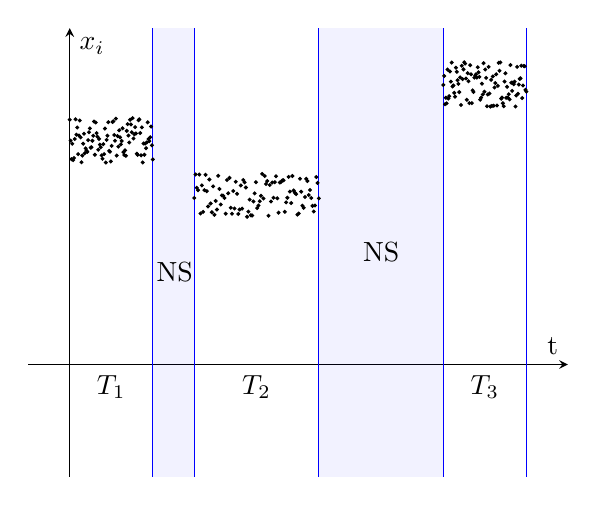
\begin{tikzpicture}
\begin{axis}[
      xlabel=t,
      ylabel=$x_i$,
      samples=100,
    xmin=-1, xmax=12,
    ymin=-1, ymax=3,
    axis lines=middle,
    ticks = none,
    ]

\addplot[only marks,domain=0:2,mark size=0.5pt]{2+0.2*rand};
\node at (axis cs:1,-0.2) [] {$T_1$};

\addplot [mark=none,blue,name path = l1] coordinates {(2, -1) (2, 3)};
\addplot[mark=none,blue,name path = l2] coordinates {(3, -1) (3, 3)};
\node at (axis cs:3.2,1) [anchor=north east] {NS};
\addplot [blue,fill opacity=0.05] fill between[of=l1 and l2];

\addplot[only marks,domain=3:6,mark size=0.5pt]{1.5+0.2*rand};
\node at (axis cs:4.5,-0.2) [] {$T_2$};

\addplot[mark=none,blue,name path = l3] coordinates {(6, -1) (6, 3)};
\addplot[mark=none,blue,name path = l4] coordinates {(9, -1) (9, 3)};
\node at (axis cs:7.5,1) [] {NS};
\addplot [blue,fill opacity=0.05] fill between[of=l3 and l4];


\addplot[only marks,domain=9:11,mark size=0.5pt]{2.5+0.2*rand};
\node at (axis cs:10,-0.2) [] {$T_3$};

\addplot[mark=none,blue] coordinates {(11, -1) (11, 3)};

\end{axis}

\end{tikzpicture}
\caption{Évolution d'une mesure $x_i$}
\label{fig:examplemesure}
\end{figure}



Chaque échantillon de mesures peut être utilisé pour calculer un échantillon d'indicateurs.
L'évolution d'un indicateur $\rho_i$ est montré dans la figure \ref{fig:exampleindicator}.

\begin{figure}[H]
\centering
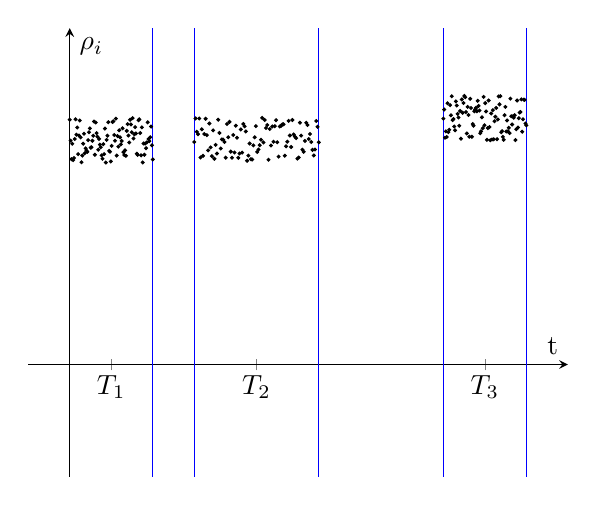
\begin{tikzpicture}
\begin{axis}[
      xlabel=t,
      ylabel=$\rho_i$,
      samples=100,
    xmin=-1, xmax=12,
    ymin=-1, ymax=3,
    axis lines=middle,
    xtick={1,4.5,10},
    ytick={\empty},
    xticklabels={\empty},
    ]

\addplot[only marks,domain=0:2,mark size=0.5pt]{2+0.2*rand};
\node at (axis cs:1,-0.2) [] {$T_1$};

\addplot [mark=none,blue,name path = l1] coordinates {(2, -1) (2, 3)};
\addplot[mark=none,blue,name path = l2] coordinates {(3, -1) (3, 3)};


\addplot[only marks,domain=3:6,mark size=0.5pt]{2+0.2*rand};
\node at (axis cs:4.5,-0.2) [] {$T_2$};

\addplot[mark=none,blue,name path = l3] coordinates {(6, -1) (6, 3)};
\addplot[mark=none,blue,name path = l4] coordinates {(9, -1) (9, 3)};



\addplot[only marks,domain=9:11,mark size=0.5pt]{2.2+0.2*rand};
\node at (axis cs:10,-0.2) [] {$T_3$};

\addplot[mark=none,blue] coordinates {(11, -1) (11, 3)};

\end{axis}

\end{tikzpicture}
\caption{Évolution d'un indicateur $\rho_i$}
\label{fig:exampleindicator}
\end{figure}

Comme les mesures dans chaque fenêtre SS ont la même espérance, les indicateurs calculés par ces mesures ont aussi la même espérance.
L'espérance de la moyenne des valeurs des indicateurs d'une fenêtre SS est identique à l'espérance des échantillons des indicateurs de cette fenêtre. 
En faisant l'hypothèse que les échantillons d'indicateurs sur une fenêtre temporelle $T_i$  sont issus d'une distribution gaussienne, la moyenne des valeurs de ces échantillons est aussi issue d'une distribution gaussienne avec une variance plus faible.
 
Dans la suite, les moyennes des indicateurs sont utilisées pour suivre l'état de santé des équipements. 
Notons $r_i$ la moyenne des valeurs de $\rho_i$ sur une fenêtre SS.
$r_i$ peut aussi décomposé en deux parties : 
\begin{equation}
    r_i  = \mu_i + \epsilon_i
\end{equation}
$\epsilon_i$ suit une distribution gaussienne d'une espérance nulle.

La valeur de $r_i$ calculée en utilisant les valeurs des échantillons de $\rho_i$ dans la fenêtre $T_j$ est notée $r_i(t_j)$, où $t_j$ est l'instant au milieu de la fenêtre temporelle $T_j$.
Les moyennes des indicateurs de la figure \ref{fig:exampleindicator} sont indiqués dans la figure \ref{fig:exampleindicateurmoyen}. Les points représentent (de gauche à droite) $r_i(t_1)$, $r_i(t_2)$, $r_i(t_3)$




  

\begin{figure}[H]
\centering
\begin{tikzpicture}
\begin{axis}[
      xlabel=t,
      ylabel=$r_i$,
      samples=100,
    xmin=-1, xmax=12,
    ymin=-1, ymax=3,
    axis lines=middle,
    xtick={1,4.5,10},
    xticklabels={$t_1$,$t_2$,$t_3$},
    ytick={\empty},
    ]

\addplot[only marks,mark size=2pt] coordinates {(1, 2)};


\addplot [mark=none,blue,name path = l1] coordinates {(2, -1) (2, 3)};
\addplot[mark=none,blue,name path = l2] coordinates {(3, -1) (3, 3)};


\addplot[only marks,mark size=2pt] coordinates {(4.5, 2)};


\addplot[mark=none,blue,name path = l3] coordinates {(6, -1) (6, 3)};
\addplot[mark=none,blue,name path = l4] coordinates {(9, -1) (9, 3)};



\addplot[only marks,mark size=2pt] coordinates {(10, 2.5)};


\addplot[mark=none,blue] coordinates {(11, -1) (11, 3)};

\end{axis}

\end{tikzpicture}
\caption{Évolutions des valeurs moyennes des indicateurs}
\label{fig:exampleindicateurmoyen}
\end{figure}

La composante déterministe des valeurs d'indicateurs évolue en présence de dégradation et de défaut. 
En représentant plus d'échantillons, nous pouvons constater l'évolution des valeurs d'indicateurs $\mathbf{r}$. 
Rappelons que l'intervalle des deux échantillons consécutives n'est pas constant. 
La ligne rouge représente l'évolution de la composante déterministe. 
Dans l'intervalle $\left[0,t_{c1}\right]$, la composante déterministe de la valeur de l'indicateur $r_i$ est constante.
C'est dans le cas où il n'y a pas de dégradation et pas de défauts brusques. 

Dans l'intervalle $\left[t_{c1},t_{c2}\right]$, la composante déterministe est continue.
On suppose que le système est en dégradation.

Aux instants $t_{c2}$ et $t_{c4}$, des changements brusques surviennent. 
L'évolution de la composante déterministe est discontinue. 
A ces instants, on suppose qu'il y a des défauts brusques surviennent.     


\begin{figure}[H]
	\centering
	\begin{tikzpicture}
	\begin{axis}[
	xlabel=$t$,
	ylabel=$r_i$,
	samples=100,
	xmin=-1, xmax=300,
	ymin=-0.2, ymax=1,
	axis lines=middle,
	xtick={50,120,140,200},
	xticklabels={$t_{c1}$,$t_{c2}$,$t_{c3}$,$t_{c4}$},
	ytick={\empty},
	]
	
	
	\addplot[only marks] table {r1.txt};
	\addplot[smooth,red,line width=3pt] table {mu1.txt};
	
	
%	\addplot[mark=none,blue,name path = l3] coordinates {(50, \pgfkeysvalueof{/pgfplots/ymin}) (50, \pgfkeysvalueof{/pgfplots/ymax})};
%	\addplot[mark=none,blue,name path = l3] coordinates {(120, \pgfkeysvalueof{/pgfplots/ymin}) (120, \pgfkeysvalueof{/pgfplots/ymax})};
%	\addplot[mark=none,blue,name path = l3] coordinates {(140, \pgfkeysvalueof{/pgfplots/ymin}) (140, \pgfkeysvalueof{/pgfplots/ymax})};
%	\addplot[mark=none,blue,name path = l3] coordinates {(200, \pgfkeysvalueof{/pgfplots/ymin}) (200, \pgfkeysvalueof{/pgfplots/ymax})};
	
	\end{axis}
	
	\end{tikzpicture}
	\caption{Évolution des valeurs d'indicateurs (points noires) et sa composante déterministe (ligne rouge)}
	\label{fig:evolutionr1bis}
\end{figure}

Comme les indicateurs peuvent être influencés par les mêmes défauts, leurs évolutions peuvent être corrélées. 
Afin d'exploiter ces corrélations nous analysons les indicateurs dans l'espace des indicateurs.
Les informations temporelles sont conservées sous la forme d'une \textit{étiquette} attachée à chaque échantillon d'indicateur.
Il peut y avoir plusieurs indicateurs.
A titre d'exemple, l'évolution d'un deuxième indicateur est simulée. 


\begin{figure}[H]
	\centering
	\begin{tikzpicture}
	\begin{axis}[
	xlabel=$t$,
	ylabel=$r_j$,
	samples=100,
	xmin=-1, xmax=300,
	ymin=-0.2, ymax=1,
	axis lines=middle,
	xtick={50,120,140,200},
	xticklabels={$t_{c1}$,$t_{c2}$,$t_{c3}$,$t_{c4}$},
	ytick={\empty},
	]
	
		\addplot[only marks] table {r2.txt};
	\addplot[smooth,red,line width=3pt] table {mu2.txt};
	
	\end{axis}
	
	\end{tikzpicture}
	\caption{Exemple de trajectoires de deux indicateurs}
	\label{fig:evolutionr2bis}
\end{figure}

La composante déterministe théorique  des deux indicateurs, qui est représentée dans l'espace d'l'indicateur, constitue des trajectoire. 
La définition d'une trajectoire est donnée ci-dessous. 
\begin{definition}
	Nous appelons une \textbf{trajectoire} l'évolution continue de la composante déterministe des valeurs d'indicateurs dans l'espace des indicateurs.
\end{definition}

Des trajectoires sont représentées dans la figure \ref{label}. 
Il existe trois trajectoires, qui sont respectivement colorées noire, bleue et rouge.  

\begin{figure}[H]
	\centering
	\begin{tikzpicture}
	\begin{axis}[
	xlabel=$\mu_i$,
	ylabel=$\mu_j$,
	samples=100,
	xmin=-0.1, xmax=0.5,
	ymin=-0.1, ymax=0.7,
	axis lines=middle,
	ticks = none
	]
	
	\addplot[smooth,line width = 1pt] table {traj1.txt};
	\addplot[smooth,blue,line width = 1pt] table {traj2.txt};
	\addplot[only marks,red,mark size=1pt] table {traj3.txt};
%	\draw
%	(axis cs:3, 2.5) coordinate (tmp) % start point
%	++(-30:5mm)
%	node[
%	below right,
%	align=left,
%	] (test) {Trajectoire 1}
%	(test.north) -- (tmp);
	

%	\draw
%	(axis cs:9, 1.5) coordinate (tmp) % start point
%	++(-30:5mm)
%	node[
%	below left,
%	align=left,
%	] (test) {Trajectoire 2}
%	(test.north) -- (tmp);
	\end{axis}
	
	\end{tikzpicture}
	\caption{Exemple de trajectoires de deux indicateurs}
	\label{fig:trajectoiremu}
\end{figure}

Cependant, comme cela a été présenté ci-dessous, ce sont les valeurs d'indicateur qui comprend à la composante aléatoire et déterministe qui sont disponibles.
Les échantillons d'indicateurs sont discrètes et l'intervalle des échantillons n'est pas une constante. 

Les valeurs de ces indicateurs sont présentées dans la figure \ref{fig:exampletrajectoirer}.

\begin{figure}[H]
	\centering
	\begin{tikzpicture}
	\begin{axis}[
xlabel=$r_i$,
ylabel=$r_j$,
samples=100,
xmin=-0.1, xmax=0.5,
ymin=-0.1, ymax=0.7,
axis lines=middle,
ticks = none
]

\addplot[only marks,mark size = 1pt] table {traj1R.txt};
\addplot[only marks,blue,mark size = 1pt] table {traj2R.txt};
\addplot[only marks,red,mark size=1pt] table {traj3R.txt};

\end{axis}
	
	\end{tikzpicture}
	\caption{Exemple d'évolution des deux indicateurs}
	\label{fig:exampletrajectoirer}
\end{figure}

\begin{itemize}
    \item présenter les valeurs discrètes dans l'espace des indicateurs
    \item Dire les contraintes pour distinguer automatiquement les évolutions causées par des dégradations et des défauts
\end{itemize}


 



\end{document}
